% Manuscript source.
\documentclass[11pt]{article}
\pagestyle{plain}
\usepackage[margin=1in]{geometry}
\usepackage{amsmath,amssymb,amsthm}
\usepackage{booktabs,longtable,array}
\usepackage{enumitem}
\usepackage[title]{appendix}
\usepackage{tikz}
\usepackage[obeyspaces,spaces,hyphens]{url}
\usepackage{xr-hyper}
\usepackage[colorlinks=true,linkcolor=blue,citecolor=blue,urlcolor=blue]{hyperref}
\usepackage{xcolor}
\usepackage[no-math]{fontspec}
\usepackage{fvextra}
\setmonofont{DejaVu Sans Mono}[Scale=MatchLowercase]

\newtheorem{theorem}{Theorem}
\newtheorem{lemma}[theorem]{Lemma}
\newtheorem{proposition}[theorem]{Proposition}
\newtheorem{corollary}[theorem]{Corollary}
\newtheorem{fact}[theorem]{Fact}
\newtheorem*{maintheorem}{Main Theorem}
\theoremstyle{definition}
\newtheorem{definition}[theorem]{Definition}
\newtheorem{computation}[theorem]{Certified computation}
\theoremstyle{remark}
\newtheorem{remark}[theorem]{Remark}

\newcommand{\R}{\mathbb{R}}
\newcommand{\Q}{\mathbb{Q}}
\newcommand{\VF}{\mathrm{VF}}
\newcommand{\aff}{\operatorname{aff}}
\newcommand{\conv}{\operatorname{conv}}
\newcommand{\relint}{\operatorname{relint}}
\newcommand{\Sym}{\operatorname{Sym}}
\newcommand{\Stab}{\operatorname{Stab}}
\newcommand{\spn}{\operatorname{span}}
\newcommand{\ch}{\operatorname{ch}}
\makeatletter
\g@addto@macro\UrlBreaks{\do\_\do\-\do\,\do\;\do\.\do\=\do\/}
\makeatother
\newcommand{\file}[1]{\path{#1}}
\setlength{\emergencystretch}{3em}

\title{The convex uniform 5-polytopes:\\ a computer-assisted classification}
\author{P. Graham\\ \small\url{https://orcid.org/0009-0007-8493-1505}}
\hypersetup{pdfauthor={P. Graham},
  pdftitle={The convex uniform 5-polytopes: a computer-assisted classification}}
\date{October 25, 2026}

\begin{document}
\maketitle
\begin{abstract}
We prove completeness of the convex uniform 5-polytope list, conditional
on the cited lower-dimensional classifications, the written reductions and
the certificate checkers. Its members are Wythoff's constructions of types
$A_5$, $B_5$, $D_5$, prisms over uniform 4-polytopes, and products of regular
polygons with uniform polyhedra. Conway and Guy announced the four-dimensional classification; Möller
gave a complete computer-assisted proof. We extend his neighborhood and
radius methods to dimension five. Coxeter's and Johnson's constructions
supply the known families. Unbounded polygon sizes require products, forced by neighbor distances and prism cells. Lean checks a conditional implication from explicit premises.
\end{abstract}

\section{Introduction}\label{sec:intro}\label{sec:models}
All polytopes are convex. Uniform polygons are regular; in higher
dimensions uniformity means vertex transitivity and uniform facets.
All edges have unit length. Write $\{p\}$ for a regular polygon,
$\{\}=[0,1]$, $P_q=\{q\}\times\{\}$, and $A_q$ for an antiprism.
Coxeter and antiprism subscripts mean rank and polygon size, respectively.

\begin{maintheorem}\label{thm:main}
Assume Facts~\ref{fact:3d} and~\ref{fact:4d}.
Every convex uniform 5-polytope is congruent, after scaling to unit edges,
to one of the following:
\begin{enumerate}[label=\textup{(K\arabic*)},leftmargin=3em]
\item a Wythoffian polytope $W_J$ of one of the Coxeter groups $A_5$,
  $B_5$, $D_5$ (19 distinct $A_5$ forms, 31 $B_5$ forms
  and 8 further $D_5$ forms);
\item a prism $K\times\{\}$ over a convex uniform 4-polytope $K$;
  45 Wythoffian bases, plus the snub 24-cell and grand antiprism, give 47
  prisms, of which 46 are not already in (K1), since the tesseract prism
  is the 5-cube;
\item a product $\{p\}\times Q$ of a regular polygon, $p\ge3$, with a
  convex uniform polyhedron $Q$: a Platonic or Archimedean solid, a prism
  $P_q$ (giving the \emph{duoprism prisms}
  $\{p\}\times\{q\}\times\{\}$), or an antiprism $A_q$.
\end{enumerate}
\end{maintheorem}
The proof below uses written reductions and certified computations; the formal theorem takes their conclusions as parameters.
\begin{definition}[Wythoffian polytopes {\cite{Wythoff1918,Coxeter1935}}]\label{def:wythoff}
Let $W$ be a finite irreducible Coxeter group of rank $k$ acting on
$\R^k$, with simple roots $\alpha_0,\dots,\alpha_{k-1}$ (nodes of the
Coxeter diagram), and let $\emptyset\ne J\subseteq\{0,\dots,k-1\}$ (the
\emph{ringed} nodes). Let $x_J$ be the point at distance $1/2$ from the
mirrors of the ringed nodes and on the mirrors of the others, on the
positive side of all of them. The \emph{Wythoffian polytope}
$W_J=\conv(W x_J)$ is uniform with unit edges. We name it by the group and
the ring pattern, e.g.\ $B_5$ \texttt{00001}; node orders are those of
Table~\ref{tab:names} in Appendix~\ref{app:names}.
\end{definition}
\begin{fact}[3-D classification {\cite[Section 18.5]{Schulte2017}, \cite{Grunbaum2009}}]\label{fact:3d}
A convex uniform polyhedron is a Platonic solid, one of the 13
Archimedean solids, a prism $P_q$ ($q\ge3$) or an antiprism $A_q$
($q\ge4$). It is determined up to congruence by its vertex configuration
(the cyclic sequence of polygon sizes around a vertex). In particular a
convex uniform polyhedron with a $q$-gonal face, $q\notin\{3,4,5,6,8,10\}$,
is $P_q$ or $A_q$.
\end{fact}
\begin{fact}[4-D classification {\cite{ConwayGuy1965,Moller2004thesis}}]\label{fact:4d}
A convex uniform 4-polytope is one of: the Wythoffians of $A_4$, $B_4$,
$D_4$, $F_4$, $H_4$; the snub 24-cell; the grand antiprism; a prism
$Q\times\{\}$ over a convex uniform polyhedron $Q$; a duoprism
$\{p\}\times\{q\}$. In particular a convex uniform 4-polytope with a
$q$-gonal 2-face, $q\notin\{3,4,5,6,8,10\}$, is a duoprism
$\{q\}\times\{p\}$ (including $P_q\times\{\}=\{q\}\times\{4\}$) or the
antiprism prism $A_q\times\{\}$.
\end{fact}
The configuration and large-polygon clauses follow by inspecting these lists.

Möller's complete four-dimensional proof \cite[Section 1.1]{Moller2004thesis}
and its published account \cite{Moller2004} follow Conway--Guy's announcement
\cite[pp.~38--39]{ConwayGuy1965}. His radius calculations, edge neighborhoods
and vertex completion \cite[Chapters 4--7 and 9]{Moller2004thesis}
are our foundation. Finite neighborhood enumeration cannot bound polygon
sizes. Our additional argument forces products for all large sizes.
Schulte reports a complete list only for $d=4$
\cite[Section 18.5]{Schulte2017}; Winter records as unknown whether
``there exist non-prismatic non-Wythoffian uniform polytopes in dimension
five or above'' \cite[Appendix E.3, p.~167]{Winter2021}.

The Open Problem Garden also lists the five-dimensional enumeration question \cite{OPG}.

\paragraph{Proof overview.}
Facet cycles fix radii; completing incident facets determines the bounded cases. For large polygons, distance bounds
leave one polygon or two sharing a duoprism at each vertex.
Their prism cells propagate translates and force products.

The proofs, the Lean formalization and the text were produced by AI models
(from OpenAI and Anthropic), working under the author's direction.
This computer-assisted work has not yet been reviewed by experts.

\section{Local geometry}\label{sec:prelim}
We relate angles, radius and neighbors.
Let $P$ be five-dimensional, with centroid $c$ and circumradius $R$.
Face centers are the orthogonal projections of $c$
(Lemma~\ref{lem:sphere}).

\begin{lemma}[Separation lemma]\label{lem:sep}
Let $X$ be a convex polytope inscribed in a sphere, with at least three
vertices, let $v$ be a vertex and $w$ a vertex nearest to $v$ among the
other vertices. Then $[v,w]$ is an edge of $X$. Consequently, in a convex
uniform polytope with unit edges any two distinct vertices are at distance
at least $1$.
\end{lemma}
\begin{proof}
The diameter ball of $[v,w]$ contains no other vertex.
Subtracting its power function from the circumsphere's gives a supporting
affine function vanishing exactly at $v,w$.
\end{proof}

For a $p$-gonal face $G$ with center $o_G$, put $\rho=r_p=1/(2\sin(\pi/p))$.
In its plane's orthogonal complement $N$, incident cells (3-faces)
give cyclic rays $u_{C_i}$; consecutive cells bound a facet with
dihedral angle $\alpha_i$.

\begin{lemma}[Closure equation]\label{lem:closure}
With this notation, let $w=c-o_G\in N$, $h=|w|=\sqrt{R^2-\rho^2}$, and for
each cell $C\supset G$ of circumradius $R_C$ let
$d_C=\sqrt{R_C^2-\rho^2}>0$. Then:
\begin{enumerate}[label=\textup{(\alph*)}]
\item $\sum_i\alpha_i<2\pi$;
\item $w\cdot u_C=d_C$, so the angle $\delta_C$ between $w$ and $u_C$
  satisfies $\cos\delta_C=d_C/h$;
\item $w$ lies strictly inside the cone spanned by the $u_C$, and with
  $\theta_i\in(0,\pi)$ the angle at $\hat w=w/h$ of the spherical triangle
  $(\hat w,u_{C_{i-1}},u_{C_i})$,
  \[
  \cos\theta_i=\frac{\cos\alpha_i-\cos\delta_{C_{i-1}}\cos\delta_{C_i}}
  {\sin\delta_{C_{i-1}}\sin\delta_{C_i}},\qquad
  \sum_{i=1}^k\theta_i=2\pi;
  \]
\item $R>R_{K}$ for every facet $K\supset G$.
\end{enumerate}
\end{lemma}
\begin{proof}
The spherical section has perimeter below $2\pi$. Projection gives (b).
The interior direction partitions the full angle into spherical triangles;
their cosine rule gives (c). Positive distance to the facet gives (d).
\end{proof}

The vertex figure $\VF$ is the neighbors' convex hull, of radius
$\sqrt{1-1/(4R^2)}$. Its edges have lengths $\ch_p=2\cos(\pi/p)$.
A \emph{star} consists of the full incident facets.
Fix $R$, the center and a facet's base vertex and neighbors.
These span and fix the full facet. Across a cell, convexity fixes the next
hyperplane; its ordered correspondence and center fix the isometry.
Traversal fixes the star (Lemma~\ref{lem:rooted}).
If each neighbor's star is forced, transporting by vertex symmetries
and inducting along the connected edge graph identifies $P$
\cite{Balinski1961} (Lemma~\ref{lem:induction}).

\section{Bounded polygon sizes}\label{sec:caseA}\label{sec:known}
Assume all polygons have at most 16 sides. Let $\mathcal K_{16}$ be (K1)--(K3) with polygon sizes at most 16.

\begin{theorem}[Case A]\label{thm:A}
Every convex uniform 5-polytope all of whose 2-faces have at most 16 sides
is congruent to one of the 628 distinct polytopes of the list $\mathcal
K_{16}$ of Section~\ref{sec:known} (all members of (K1)--(K3) whose
polygons have at most 16 sides).
\end{theorem}
\begin{proof}
The classifications give a finite facet list.
The closure equation enumerates cyclic facet words with angle sum at most
$2\pi$. Remove exact flat and degenerate cases; let $\Omega$ be the union
of remaining radius intervals (Computation~\ref{comp:S1}). Overlap components collect possible common
radii. Repeatedly remove cycles missing a required facet incidence.
A cycle of $P$ remains: every polygon orbit of a facet occurs through
its base vertex (Lemma~\ref{lem:filter}).

Fix the least facet and its position. Every continuation across a ridge
has the same cell label, some ordered correspondence and the opposite
hinge. Exhaust these possibilities, identifying only exact isometries.
Strict separation, support or incidence contradictions exclude cases;
uncertain cases remain (Lemma~\ref{lem:equiv}).
Computation~\ref{comp:S2} leaves 629 signatures, the multisets of facet types and cyclic edge words.

The closure function is the angle sum minus $2\pi$, parametrized by reciprocal radius. For each signature it changes sign at the interval
endpoints and has derivative excluding zero throughout, giving a unique radius (Computation~\ref{comp:root}). Every actual star has a represented ordered encoding.
For each known construction, exact exclusions eliminate every
other encoding; its existence supplies the star.
Fixed-radius rigidity identifies it. Every continuation at a neighbor
then gives that same star, hence that polytope.

The remaining signature has eight neighbors and $R=1$.
Its unique encoding forces the first neighbor's star; at the second,
none of the 48 congruences contains all known facets.
Thus it cannot occur (Computation~\ref{comp:dev}). The enumeration gives 629 signatures: 628 known polytopes and this one refuted case.\end{proof}

\section{Large polygons}\label{sec:caseB}
A large polygon has at least 17 sides. This exceeds the exceptional sizes
in Facts~\ref{fact:3d}--\ref{fact:4d} and satisfies $2\sin(2\pi/17)<1$.
At each vertex there are $s$ large polygons, by transitivity.
Each gives a long VF-edge $e$; its \emph{fan} comprises the VF-facets containing it.

\begin{lemma}[Long edges are disjoint]\label{lem:long}
Two long VF-edges share no vertex.
\end{lemma}
\begin{proof}
Endpoints opposite a shared endpoint would lie within $2\pi/17$ of
its antipode, hence less than one apart.
\end{proof}

The angle sum allows three cycle types:
(i) duoprisms $\{n\}\times\{q_i\}$ with three to five rays;
(ii) two $A_n\times\{\}$ and one duoprism;
(iii) two $A_n\times\{\}$ and two duoprisms, with pairs
$(3,3),(3,4),(3,5)$.
Indeed an antiprism ray costs two right angles; none or one occurs.
At least one duoprism is necessary; two require
$1/q_1+1/q_2>1/2$; three exceed the angle sum.

For type (i), lateral unit vectors satisfy $u_i\cdot(c-o_G)=1/2$.
Their circle radius $S\in(\max_i\cos(\pi/q_i),1)$ uniquely solves
\[
 \sum_i2\arcsin(\cos(\pi/q_i)/S)=2\pi,\quad
 R_c^2=\frac1{4(1-S^2)},\quad R^2=r_n^2+R_c^2.
\]
For (ii) and (iii), with antiprism height
$h_A(n)^2=1-1/(4\cos^2(\pi/(2n)))$, projection gives respectively
\[
 R^2=R_{A_n}^2+r_q^2,\qquad
 R^2=R_{A_n}^2+\frac1{2(1+\gamma)},\qquad R_{A_n}^2=r_n^2+h_A(n)^2/4.
\]
Here $\gamma$ is the cosine between the two lateral prism rays.
The radius certificates separate these from $\Omega$:
the finite check ends at 397, and $r_{398}>\max\Omega$ covers every tail.

\begin{corollary}\label{cor:B2}
Every 2-face $G$ of $P$ lies in a large facet. Consequently every VF-edge
at $v$ lies in a VF-facet $\VF(K)$ with $K$ large, and $K$ contains a large
2-face through $v$.
\end{corollary}
\begin{proof}
Otherwise its small-facet cycle puts $R$ in $\Omega$, contradicting
the radius forced by a large polygon. Every vertex of a large facet
lies on a large polygon.
\end{proof}

A fan is \emph{paired} if a facet contains another large polygon.
Configuration-radius comparisons exclude 67 unpaired configurations.
The fan distance certificates bound pairs of admissible points, meaning
points on the VF sphere satisfying the fan's supporting inequalities
and separation from its vertices.

\begin{lemma}\label{lem:Wuse}
Let $F$ be a large 2-face at $v$ whose fan is in the list of
Computation~\ref{comp:W} (with the actual $n$, $m$ of $P$). Then the only
long VF-edges with an end among the fan vertices or an admissible point
are $e$ and, for a paired fan, the partner edge. In particular every long
VF-edge is $e$ or the partner edge.
\end{lemma}
\begin{proof}
Disjointness excludes distinguished endpoints.
The distance certificates leave only pairs of fan vertices.
Other pairs are short or polygon diagonals. The lateral vertices lie on
a circle in fan order; a diagonal crosses another diagonal internally,
so cannot be a VF-edge. For three vertices there is no diagonal.
\end{proof}

Seven paired fans need $n=m$. Put
$\delta_{c_1}(m)=R_{(m,c_1)}^2-r_m^2$.
The partner cycle gives
\[
 R^2=r_n^2+r_m^2+\delta_{c_1}(m),\quad
 \delta_{c_1}(m)=\delta_{c_2}(n)\ \text{or}\ h_A(m)^2/4.
\]
Finite comparison forces equality of parameters
(Lemma~\ref{lem:partner}), bringing these fans under the distance bound.
\begin{proposition}\label{prop:reduction}
If $s\ge2$, then $s=2$ and the two large 2-faces $F_1$ ($n$-gon) and $F_2$
($m$-gon) at $v$ lie in a common facet $D=\{n\}\times\{m\}$.
\end{proposition}
\begin{proof}
An unpaired fan permits only its distinguished long edge; a paired fan
permits exactly it and its partner. Their common facet is the duoprism.
\end{proof}

\begin{fact}[F3]\label{fact:F3}
In $\{n\}\times\{q\}$ and in $A_n\times\{\}$ every vertex lies on an
$n$-gon. At a vertex $v$:
$\VF(\{n\}\times\{q\})$ is the tetrahedron $\conv(a,b,g,g')$, where $a,b$
are the neighbors on the $n$-gon and $g,g'$ those on the $q$-gon:
$|ab|=\ch_n$, $|gg'|=\ch_q$, $ab\perp gg'$, and the other four edges have
length $\sqrt2$. $\VF(A_n\times\{\})$ is the pyramid with apex $z$ (the
prism edge) over the trapezoid $(a,b,y,x)=\VF(A_n)$: $ab$ is the VF-edge of
the $n$-gon, $|by|=|yx|=|xa|=1$ (the three triangles at $v$), the diagonals
$ay$, $bx$ have length $\sqrt{1+\ch_n}$, and the four apex edges have
length $\sqrt2$.
\end{fact}
\begin{proof}Product neighbors give these lengths, incidences and orthogonality.\end{proof}

\begin{figure}[ht]
\centering
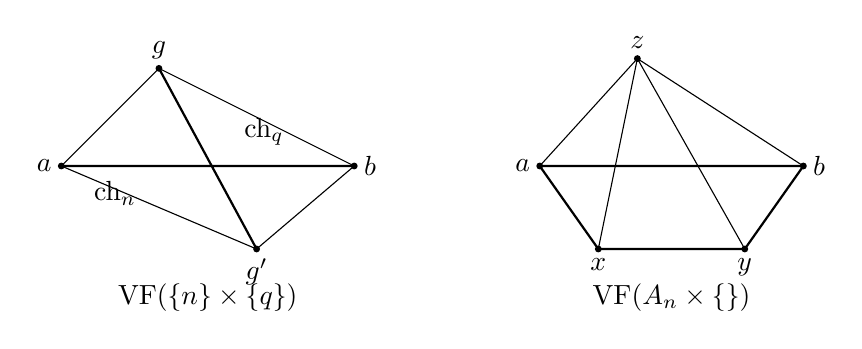
\begin{tikzpicture}[scale=.62]
\coordinate (a) at (-3,0); \coordinate (b) at (3,0);
\coordinate (g) at (-1,2); \coordinate (h) at (1,-1.7);
\draw (a)--(g)--(b)--(h)--(a);
\draw[thick] (a)--(b) (g)--(h);
\node[below] at (-1.9,-.12) {$\ch_n$};
\node[right] at (.55,.7) {$\ch_q$};
\fill (a) circle (2pt) node[left] {$a$};
\fill (b) circle (2pt) node[right] {$b$};
\fill (g) circle (2pt) node[above] {$g$};
\fill (h) circle (2pt) node[below] {$g'$};
\node at (0,-2.7) {$\VF(\{n\}\times\{q\})$};
\begin{scope}[xshift=9.5cm]
\coordinate (aa) at (-2.7,0); \coordinate (bb) at (2.7,0);
\coordinate (x) at (-1.5,-1.7); \coordinate (y) at (1.5,-1.7);
\coordinate (z) at (-.7,2.2);
\draw[thick] (aa)--(bb)--(y)--(x)--(aa);
\draw (z)--(aa) (z)--(bb) (z)--(y) (z)--(x);
\fill (aa) circle (2pt) node[left] {$a$};
\fill (bb) circle (2pt) node[right] {$b$};
\fill (x) circle (2pt) node[below] {$x$};
\fill (y) circle (2pt) node[below] {$y$};
\fill (z) circle (2pt) node[above] {$z$};
\node at (0,-2.7) {$\VF(A_n\times\{\})$};
\end{scope}
\end{tikzpicture}
\caption{The two vertex figures of Fact~\ref{fact:F3}, drawn schematically.
Left: the tetrahedron, with orthogonal distinguished chords.
Right: the pyramid over the antiprism's trapezoid; $ab$ is the long edge.}
\label{fig:duoprism}
\end{figure}
\begin{theorem}\label{thm:s1}
If $s=1$, then $P\cong\{n\}\times Q$ for a convex uniform polyhedron $Q$,
or $P\cong A_n\times\{q\}$.
\end{theorem}

Fix $v$, its large 2-face $F$ (an $n$-gon with plane direction $L$) and
$e=[a,b]$ its VF-edge. By Corollary~\ref{cor:B2} and $s=1$, every VF-edge
lies in a VF-facet $\VF(K)$ with $K\supset F$; so \emph{every VF-edge, and
hence every VF-vertex, lies in a facet of the fan of $e$}. The fan is
given by the cycle type of $F$ (Lemma~\ref{lem:F5}).

\begin{proof}[Type (i)]
The fan facets are $T_i=\conv(a,b,x_i,x_{i+1})$, where $[v,x_i]$ is the
lateral edge of the $i$-th cell $F\times[v,x_i]$; so $x_i-v\perp L$, and the
neighbors of $v$ are exactly $a,b,x_1,\dots,x_k$. Distinct prism cells give distinct lateral edges.

\emph{Product lemma.} For a vertex $t$ let $F_t$ be its unique large
2-face. Transitivity gives the same local picture at $t$, carrying $F$ to $F_t$. For a
neighbor $t'$ of $t$, either $t'\in F_t$, and then $F_{t'}=F_t$; or $t'-t$
is a lateral edge, orthogonal to the plane of $F_t$, and the duoprism
$\{n\}\times\{q_i\}$ containing the edge $tt'$ contains the translate
$F_t+(t'-t)$, a large 2-face at $t'$, so $F_{t'}=F_t+(t'-t)$. The edge graph of $P$ is connected
\cite{Balinski1961}, so every $F_t$ is a translate $F+\tau_t$ with
$\tau_t\perp L$ (each step adds $0$ or a vector orthogonal to $L$).
Hence the vertex set is $F_0+X$, with $F_0$ the polygon $F$ centered at the
origin of $L$ and $X$ a finite set in an affine copy of $L^\perp$, and
$P=\conv F_0+\conv X\cong\{n\}\times Q$ with $Q=\conv X$, a 3-polytope since
$\dim P=5$. A product point is a vertex exactly when both coordinates are vertices, so $X=\operatorname{Vert}Q$. Product faces give $Q$ unit edges and regular faces. Symmetries preserve the unique polygon plane $L$, hence $L^\perp$, and induce a transitive isometry group on $Q$. Thus $Q$ is uniform.
\end{proof}

\begin{proof}[Type (ii)]
The fan consists of the pyramids $\Pi_1=(z_1;a,b,y,x)$,
$\Pi_2=(z_2;a,b,y,x)$ (the two $A_n\times\{\}$ sharing the $A_n$ cell $C$,
$\VF(C)=(a,b,y,x)$) and $T=\conv(a,b,z_1,z_2)$. The neighbors of $v$ are
$a,b,x,y$ (in $C$) and $z_1,z_2$, with $z_j-v$ orthogonal to the
3-space $M$ of $C$. \emph{Cell partition:} for a vertex $t$ let $C_t$ be
the unique $A_n$ cell containing $F_t$ (one $A_n$ ray per cycle). For
$t'\in C_t$, $t'$ lies on exactly one of the two $n$-gons of $C_t$ ($n\ge4$),
which is then $F_{t'}$, so $C_{t'}=C_t$. The other two neighbors $t'$ of
$t$ satisfy $t'-t\perp M_t$, and the $A_n\times\{\}$ containing $tt'$ gives
$C_{t'}=C_t+(t'-t)$. So the vertex set is $C_0+X$ with $X$ in a 2-plane
orthogonal to $M$, $P=A_n\times\conv X$, and $\conv X$ is a
vertex-transitive equilateral convex polygon with unit edges, i.e.\ a
regular polygon $\{q\}$.
\end{proof}

\begin{proof}[Type (iii) does not occur]
The fan consists of $\Pi_1$, $\Pi_2$ as in (ii) and $T_1=\conv(a,b,z_1,w)$,
$T_2=\conv(a,b,w,z_2)$, where $w-v$ is the lateral edge of the $P_n$ cell
between the two duoprisms. The seven points $a,b,x,y,z_1,z_2,w$ are
distinct: $a-v,b-v\in L$; $x-v$ and $y-v$ are neither in $L$ nor orthogonal
to $L$ ($x,y$ lie on the other $n$-gon of the antiprism, rotated by $\pi/n$
and at height $h_A>0$), and $x\ne y$; $w-v$, $z_1-v$, $z_2-v$ are orthogonal
to $L$ and are the lateral edges of three different $P_n$ cells. Since
every VF-edge lies in a fan facet, the VF-edges are exactly the edges of
these four facets:
\[ab,\ ax,\ xy,\ yb,\ z_ja,\ z_jb,\ z_jx,\ z_jy\ (j=1,2),\ wa,\ wb,\ wz_1,\ wz_2.\]
In particular $z_1z_2$ is not a VF-edge, and $x$ has exactly the VF-edges
$xa,xy,xz_1,xz_2$, $y$ exactly $yb,yx,yz_1,yz_2$, and $w$ exactly
$wa,wb,wz_1,wz_2$; each of $x,y,w$ is simple (Lemma~\ref{lem:simple}). The
triangle $(x,y,z_1)$ is a 2-face of $\Pi_1$, hence a VF-ridge, lying in
$\Pi_1$ and exactly one other VF-facet $K'$. At $x$, $\Pi_1$ has the edges
$\{xa,xy,xz_1\}$, so $K'$ has $\{xy,xz_1,xz_2\}$; thus $xa$ is not an edge of
$K'$, and by Lemma~\ref{lem:face} $a\notin K'$. Likewise, at $y$, $b\notin
K'$. If $w$ were in $K'$, its $K'$-edges would be among $wz_1,wz_2$ (the
others go to $a,b$), degree at most 2 in a 3-polytope, impossible. So
$K'=\conv(x,y,z_1,z_2)$, a tetrahedron, and its edge $z_1z_2$ is an edge of
$\VF$ (Lemma~\ref{lem:face}, converse), which it is not.
\end{proof}

\begin{theorem}\label{thm:paired}
If every vertex lies in exactly two large 2-faces $F_1$ ($n$-gon) and $F_2$
($m$-gon), and they lie in a common facet $D=\{n\}\times\{m\}$, then $P$ is
$\{n\}\times\{m\}\times\{\}$, $A_m\times\{n\}$ or $A_n\times\{m\}$.
\end{theorem}

\begin{proof}
Let $e_1=[a,b]$ and $e_2=[c,d]$ be the VF-edges of $F_1$, $F_2$; then
$\VF(D)=\conv(a,b,c,d)$. By Corollary~\ref{cor:B2} every VF-edge lies in
$\mathrm{fan}(e_1)$ or $\mathrm{fan}(e_2)$, so every VF-vertex is a vertex of
one of the two fans. The fan of $F_1$ is of type (i) with configuration
$(m,q_2,\dots,q_k)$, $x_1=c$, $x_2=d$, or of type (ii) with apexes
$\{z_1,z_2\}=\{c,d\}$ (as $T=\VF(D)$); likewise for $F_2$ with $n$. The angle
sum allows only $k=3$, or $k=4$ with configuration $(m,3,3,3)$ (the
configurations $(m,4,p,p')$ and $(m,3,p,p')\ne(m,3,3,3)$ exceed $2\pi$).

\emph{Simple-vertex step.} A vertex $z$ of $\mathrm{fan}(e_1)$ not in
$\mathrm{fan}(e_2)$ has all its VF-edges in $\mathrm{fan}(e_1)$. If it has
degree 4, each 3-subset of its edges spans a VF-facet
(Lemma~\ref{lem:simple}), and a VF-facet containing $c$ and $d$ contains
the edge $e_2$ (Lemma~\ref{lem:face}), hence belongs to $\mathrm{fan}(e_2)$.

\emph{(i)/(i), $k=3$.} $z=x_3$ has the VF-edges $za,zb,zc,zd$ in
$\mathrm{fan}(e_1)$. If $z\notin\mathrm{fan}(e_2)$, the facet spanned by
$\{za,zc,zd\}$ contains $e_2$, so $z\in\mathrm{fan}(e_2)$ after all. In a
type-(i) fan of $e_2$ every vertex other than $c,d$ is at distance $\sqrt2$
from $c$ and $d$ (Fact~\ref{fact:F3}), so
$\ch_{q_2}=|z-d|=\sqrt2=|z-c|=\ch_{q_3}$: the configuration is $(m,4,4)$. The other cases below leave only $(n,4,4)$ for $F_2$, with the same third vertex $z$. \emph{Translate argument:} for a vertex $t$ let $D_t$ be the
facet containing its two large 2-faces. For $t'\in D_t$, both large 2-faces
of $D_t$ at $t'$ are large 2-faces of $P$, so $D_{t'}=D_t$. The
$\{n\}\times\{4\}$ and $\{m\}\times\{4\}$ facets at the edge $vz$ contain
$F_1+\tau$ and $F_2+\tau$, $\tau=z-v\perp\spn D$, so $D_z=D+\tau$. Hence the
vertex set is $D_0+X$ with $X$ on a line, every point of $X$ is a vertex, so
$|X|=2$ and $P=\{n\}\times\{m\}\times\{\}$.

\emph{(i)/(i), $k=4$: both fans of type (i), that of $F_1$ with
configuration $(m,3,3,3)$.} Here
$|x_3-d|=|x_4-c|=\ch_3=1\ne\sqrt2$, so neither $x_3$ nor $x_4$ lies in a
type-(i) fan of $e_2$. Then both are simple with all edges in
$\mathrm{fan}(e_1)$: $x_3$ has $x_3a,x_3b,x_3d,x_3x_4$ and $x_4$ has
$x_4a,x_4b,x_4x_3,x_4c$. The facet $G$ at $x_3$ spanned by
$\{x_3a,x_3d,x_3x_4\}$ contains $x_4$ and $a$, hence the edge $x_4a$
(Lemma~\ref{lem:face}); it does not contain $b$ (else $x_3b$ would be a
fourth edge of $G$ at the simple vertex $x_3$). So at $x_4$ its edges are
$\{x_4a,x_4x_3,x_4c\}$, and $G$ contains $c$ and $d$, so $G\in\mathrm{fan}(e_2)$
and $x_3\in\mathrm{fan}(e_2)$, a contradiction. Impossible.

\emph{(i)/(ii).} $\mathrm{fan}(e_2)$ is the pair of $A_m\times\{\}$ with
apexes $a,b$ and trapezoid $(c,d,y',x')$, with $|dy'|=|y'x'|=|x'c|=1$ and
diagonals $\sqrt{1+\ch_m}\in[1.7222,\sqrt3)$, strictly between $\ch_5$ and
$\ch_6$, hence not a chord $\ch_q$ of any polygon. If $k=3$, $x_3$ must lie in
$\mathrm{fan}(e_2)$ (as above) at distances $\ch_{q_2}$, $\ch_{q_3}$ from $d$,
$c$; but the vertices of $\mathrm{fan}(e_2)$ other than $a,b,c,d$ are $x',y'$,
each at distance $1$ from one of $c,d$ and at the diagonal distance from the
other, and the diagonal is not a chord; impossible. If
$k=4$, $(m,3,3,3)$: by the argument of the previous case one of $x_3,x_4$
lies in $\mathrm{fan}(e_2)$; by symmetry say $x_3$; $|x_3-d|=1$ forces
$x_3=y'$. If $x_4\notin\mathrm{fan}(e_2)$, $x_4$ is simple and its facet
spanned by $\{x_4a,x_4x_3,x_4c\}$ meets the pyramid $\Pi(a;c,d,y',x')$ in a
face containing $a,c,y'$; since $c,y'$ are opposite vertices of the base, no
proper face of the pyramid contains these three, so the facet is the
pyramid and $x_4\in\mathrm{fan}(e_2)$. Hence $\{x_3,x_4\}=\{y',x'\}$ and the
neighbors of $v$ are those of $\mathrm{fan}(e_2)$. \emph{Cell partition:}
Transitivity preserves fan types, even at $n=m$; denote the unique type-(ii) antiprism cell by $C_t$. For $t'\in C_t$ the $m$-gon of $C_t$ through $t'$ has $C_t$ in its
cycle, so it is not of type (i): it is the type-(ii) 2-face at $t'$, and
$C_{t'}=C_t$. The other neighbors $a,b$ of $v$ are the apexes of
$\mathrm{fan}(e_2)$, so $a-v$ and $b-v$ are orthogonal to the 3-space of
$C_v$ and $C_a=C_v+(a-v)$. So $P=A_m\times\conv X$ with $\conv X$ a regular
polygon, here $F_1$: $P=A_m\times\{n\}$. The case (ii)/(i) gives
$A_n\times\{m\}$.

\emph{(ii)/(ii).} The trapezoid vertex $x$ of $\mathrm{fan}(e_1)$ (edges
$xa,xy,xc,xd$ in $\mathrm{fan}(e_1)$, the apexes being $c,d$) must lie in
$\mathrm{fan}(e_2)$ (otherwise the facet spanned by $\{xy,xc,xd\}$ contains
$e_2$), so $x\in\{x',y'\}$ at distance $1$ or $\sqrt{1+\ch_m}$ from $c$. But
$|x-c|=\sqrt2$, since $c$ is an apex of a prism over the $A_n$ cell
containing $x$. Impossible.
\end{proof}



\begin{proof}[Proof of the Main Theorem]
Theorem~\ref{thm:A} gives (K1)--(K3). Otherwise Proposition~\ref{prop:reduction}
leaves one large polygon, handled by Theorem~\ref{thm:s1}, or two paired
ones, handled by Theorem~\ref{thm:paired}, both giving (K3).
These constructions are convex and uniform.
\end{proof}

\section{Computational verification}\label{sec:verification}\label{sec:lean}
Exact algebra and certified intervals establish the finite assertions
\cite{Johansson2017}. Checking notes give certificates, dependencies and commands.

With the two cited classifications and twelve geometric/computational
premises as parameters, \texttt{Uniform5.Composition.mainClassification} proves
\[
 \forall P:\operatorname{Set}(\operatorname{Space}5),\quad
 \operatorname{UnitUniform}(5,P)\Longrightarrow K_1(P)\lor K_2(P)\lor K_3(P).
\]
Here $\operatorname{Space}5=\mathbb R^5$;
$\operatorname{UnitUniform}$ means a full-dimensional finite convex hull,
vertex-transitive with recursively uniform facets and unit exposed edges.
Formal $K_1$ uses Definition~\ref{def:wythoff}; $K_2$ allows every unit uniform 4-dimensional base, including both exceptional polytopes; $K_3$ uses Fact~\ref{fact:3d}. Exposed segments are the polytope's edges. Congruence is intrinsic Euclidean congruence, with unit normalization matching the scaling convention. Lean proves the classification direction; construction uniformity and counts remain external.

Table~\ref{tab:formal-inputs} matches all twelve premise types to the mathematical conditions used above. Lean checks their conditional composition; the joint instantiation from the supplied certificates is external. The cited parameters are Facts~\ref{fact:3d}--\ref{fact:4d}. The logical axioms are standard; their list and exact declarations are in the checking notes.
\begin{appendices}
\section{Supporting geometric calculations}\label{app:geometry}
These calculations justify the local geometric formulas and placement comparisons used above. Write $V$ for the vertices of $P$, $\mathcal L_{16}$ for the finite facet list, $\mathcal C_{16}$ for its cycles, and $\mathcal K_{16}$ for the known constructions with polygon sizes at most 16. For a facet model $K$, $X_K$ is its vertex figure, of radius $r_K$; the ambient vertex figure has radius $r=\sqrt{1-1/(4R^2)}$. The group $E_K$ consists of exact center-fixing isometries of $X_K$ preserving labeled ridges.\par

\begin{lemma}\label{lem:sphere}
Let $c$ be the centroid of $V$. Then all vertices lie on the sphere of some
radius $R$ about $c$, and $c$ lies in the interior of $P$. For every face
$\Phi$ of $P$ the orthogonal projection $o_\Phi$ of $c$ onto $\aff\Phi$ is
the circumcenter of $\Phi$, and lies in the relative interior of $\Phi$.
If $\Phi$ has circumradius $R_\Phi$, then
$|c-o_\Phi|=\sqrt{R^2-R_\Phi^2}$.
\end{lemma}
\begin{proof}
Every symmetry permutes $V$ and so fixes $c$; by vertex-transitivity all
vertices are equidistant from $c$. The centroid of the vertices of a
full-dimensional polytope is an interior point. The vertices of $\Phi$ lie
on the intersection of the sphere with $\aff\Phi$, a sphere in $\aff\Phi$
about $o_\Phi$; they affinely span $\aff\Phi$, so $o_\Phi$ is the unique
circumcenter of $\Phi$. Since $\Phi$ is uniform, applying the first part to
$\Phi$ shows that its circumcenter is its vertex centroid, which is
relatively interior. The last formula is Pythagoras.
\end{proof}

\label{sec:closure}
\begin{lemma}\label{lem:vf}
Let $P$ be a convex uniform $d$-polytope with unit edges and circumradius
$R$, centered at $0$, and $v$ a vertex. The neighbors of $v$ (the other
ends of the edges at $v$) are exactly the vertices at distance $1$ from
$v$. They lie on the hyperplane $H=\{x: x\cdot v=R^2-\tfrac12\}$, every other
vertex except $v$ lies strictly on the side $x\cdot v<R^2-\frac12$, and
$\VF:=H\cap P=\conv(\text{neighbors of }v)$ is a $(d-1)$-polytope
inscribed in a sphere of radius $r=\sqrt{1-1/(4R^2)}$ about
$o_{\VF}=(1-\frac{1}{2R^2})v$. The faces of $\VF$ correspond to the faces
of $P$ containing $v$ (a $j$-face $\Phi\ni v$ gives the $(j-1)$-face
$H\cap\Phi$). For a facet $K\ni v$ of circumradius $R_K$, $\VF(K):=H\cap K$
is inscribed in a sphere of radius $r_K=\sqrt{1-1/(4R_K^2)}$ in a
hyperplane of $H$ at distance $\sqrt{r^2-r_K^2}$ from $o_{\VF}$. An edge of
$\VF$ coming from a $p$-gon has length $\ch_p=2\cos(\pi/p)$. The point
$o_{\VF}$ lies in the relative interior of $\VF$.
\end{lemma}
\begin{proof}
By Lemma~\ref{lem:sep} the vertices at distance 1 from $v$ are neighbors,
and conversely neighbors are at distance 1. For a vertex $x$,
$|x-v|^2=2R^2-2x\cdot v$, so $|x-v|=1$ iff $x\cdot v=R^2-\frac12$, and
$|x-v|>1$ (every other vertex $\ne v$) iff $x\cdot v<R^2-\frac12$. Hence $H$
separates $v$ from all non-neighbors, and $H\cap P$ is the convex hull of
the neighbors; this is the standard vertex figure, whose face lattice is
that of the faces through $v$. A neighbor $x$ makes an angle $\theta$
with $v$ at the center with $2R\sin(\theta/2)=1$, so its distance from
the axis $\R v$ is $R\sin\theta=\cos(\theta/2)=\sqrt{1-1/(4R^2)}$. The
same computation inside $K$ gives $r_K$; the circumcenter of $\VF(K)$ is
the projection of $o_{\VF}$, which gives the distance. In a regular
$p$-gon the two neighbors of a vertex are $\ch_p$ apart. Finally, write
$o_{\VF}=t_0v$ with $t_0=1-1/(2R^2)$. Since $0$ is the centroid of the $N$
vertices, $q:=-v/(N-1)$ is the centroid of the vertices other than $v$, so
$q\in P$, and $q\cdot v\le R^2-\frac12$, since every other vertex $x$ has
$x\cdot v\le R^2-\frac12$, with equality exactly for the neighbors. If some
vertex other than $v$ is not a neighbor, the inequality is strict, i.e.\
$-1/(N-1)<t_0$; also $t_0<1$. Then $o_{\VF}$ lies on the open segment from
$q$ to $v$, which passes through the interior point $0$; every point of
this open segment is interior to $P$ (it lies strictly between the
interior point $0$ and a point of $P$, or is $0$). Hence $o_{\VF}$ is an
interior point of $P$ lying in $H$, i.e.\ a relative interior point of
$\VF=H\cap P$. If every vertex other than $v$ is a neighbor (as in the
5-simplex), then $\VF$ is the convex hull of all other vertices, $t_0=-1/(N-1)$
and $o_{\VF}=q$ is the centroid of the vertices of $\VF$, which is a
relative interior point of $\VF$.
\end{proof}


\begin{lemma}[Exact exclusions]\label{lem:exclusions}
\textup{(Flat.)} A cycle with $\sum\alpha_i=2\pi$ exactly is not the cycle
of a 2-face of a convex 5-polytope. \textup{(Degenerate.)} A root at
$R=R_{\max}$ exactly does not give a convex uniform polytope.
\end{lemma}
\begin{proof}
Lemma~\ref{lem:closure}(a) and (d).
\end{proof}


\begin{lemma}[Face lemma]\label{lem:face}
Let $X$ be a polytope, $\Phi$ a face of $X$ and $p,q$ vertices of
$\Phi$. If $[p,q]$ is an edge of $X$, it is an edge of $\Phi$. Conversely
every edge of $\Phi$ is an edge of $X$.
\end{lemma}
\begin{proof}
$[p,q]\subseteq\Phi$ by convexity, and $[p,q]=[p,q]\cap\Phi$ is an
intersection of two faces of $X$, hence a face of $X$ contained in
$\Phi$, hence a face of $\Phi$. The converse holds because a face of a
face is a face.
\end{proof}


\begin{lemma}[Simple vertices]\label{lem:simple}
A vertex $x$ of degree 4 in a 4-polytope is simple: each facet containing
$x$ contains exactly three of the four edges at $x$, and each 3-subset of
the edges at $x$ is the set of edges at $x$ of exactly one facet.
\end{lemma}
\begin{proof}
The vertex figure of $x$ is a 3-polytope with four vertices, a
tetrahedron; its facets (all four triangles) correspond to the facets
through $x$.
\end{proof}


\begin{lemma}[Local uniqueness gives global uniqueness]\label{lem:induction}
Let $S$ be the star of $v_0$ in some convex uniform 5-polytope, and
suppose: for every convex uniform 5-polytope $P$ with star $S$ at $v_0$
and every neighbor $w$ of $v_0$, the star of $P$ at $w$ is one and the
same set $\Sigma_w$, independent of $P$. Then any two convex uniform
5-polytopes $P_1$, $P_2$ with star $S$ at $v_0$ are equal.
\end{lemma}
\begin{proof}
We show by induction on the edge distance from $v_0$ that $P_1$ and $P_2$
have the same vertices and the same stars there. Suppose $P_1$ and $P_2$
have the same star $\Sigma$ at a vertex $w$. By vertex-transitivity of
$P_1$ there is an isometry $g_1$ with $g_1(v_0)=w$ and $g_1(S)=\Sigma$.
Then $g_1^{-1}(P_1)$ and $g_1^{-1}(P_2)$ are convex uniform 5-polytopes
with star $S$ at $v_0$; by hypothesis they have the same star at every
neighbor $u'$ of $v_0$. Applying $g_1$, $P_1$ and $P_2$ have the same
star at every neighbor $u=g_1(u')$ of $w$ (the neighbors of $w$ are
read off the common star $\Sigma$). The edge graph of a polytope is
connected (Balinski \cite{Balinski1961}), and a polytope is the convex
hull of its vertices, so $P_1=P_2$.
\end{proof}

\label{sec:facetdata}
\begin{lemma}[A word determines its angle]\label{lem:wordangle}
Let $G$ be a $p$-gon of a uniform 4-polytope $K$ (circumradius $R_K$),
between cells $A$, $B$ of circumradii $R_A$, $R_B$, and let $\rho=r_p$.
Then the dihedral angle of $K$ at $G$ is
\[
\alpha=\arccos\sqrt{\frac{R_A^2-\rho^2}{R_K^2-\rho^2}}
      +\arccos\sqrt{\frac{R_B^2-\rho^2}{R_K^2-\rho^2}} .
\]
In particular the word $(K,p,A,B)$ determines $\alpha$, even when its
polygon occurrences lie in different orbits of $\Sym(K)$.
\end{lemma}
\begin{proof}
In the plane through the center $f$ of $G$ perpendicular to $G$, the two
cells give rays $u_A,u_B$ bounding a convex wedge of angle $\alpha$, and
the center $O$ of $K$ projects strictly inside it (Lemma~\ref{lem:sphere}
applied to $K$, and Lemma~\ref{lem:closure}(b),(c) one dimension down).
With $D=|O-f|^2=R_K^2-\rho^2$ we have $(O-f)\cdot u_A=\sqrt{R_A^2-\rho^2}>0$
and likewise for $B$, since the projection of $O$ on each cell is its
relatively interior circumcenter. The direction of $O-f$ lies between the
rays, so the two angles to it add to $\alpha$.
\end{proof}


\begin{corollary}\label{cor:omega}
Let $X$ be any convex uniform 5-polytope with unit edges and circumradius
$R_X$, and $G$ a 2-face of $X$ all of whose facets (around $G$) belong to
$\mathcal L_{16}$, with $G$ at most 16-gonal. Then $R_X$ lies in a root
interval of the cycle of $G$, and that interval belongs to $\Omega$.
\end{corollary}
\begin{proof}
The cycle of $G$ is a library cycle (Lemma~\ref{lem:closure}(a)), hence
in $\mathcal C_{16}$; it is not flat (Lemma~\ref{lem:exclusions});
$1/R_X$ is a zero of $g$ in $[0,1/R_{\max})$ by
Lemma~\ref{lem:closure}(c),(d), so it lies in a root interval, which is not
a degenerate one (Lemma~\ref{lem:exclusions}).
\end{proof}


\begin{lemma}\label{lem:filter}
All cycles of the 2-faces of $P$ at a vertex $v$ lie in one radius class,
the class containing $R$, and none of them is removed by the closure
filter.
\end{lemma}
\begin{proof}
By Corollary~\ref{cor:omega} each of these cycles has a root interval in
$\Omega$ containing $R$, so all these intervals lie in the class of $R$.
Let $K$ be a facet of $P$ at $v$ and $(p,C_a,C_b)$ a polygon orbit of $K$.
Since $K$ is vertex-transitive, the orbit has a member $G\ni v$, a 2-face
of $P$ whose cycle contains $K$ between $C_a$ and $C_b$; this cycle is in
the class of $R$. So the set of cycles of $P$'s 2-faces at $v$ is never
touched by the filter (by induction over the iterations).
\end{proof}

\label{sec:S2}\label{sec:U2}
\begin{lemma}[Exact equivalence of placements]\label{lem:equiv}
Let $g$ be an exact isometry of the model vertex figure $X_K$ fixing its
center, preserving its labeled ridges and VF-edge polygon sizes, and
mapping an ordered source ridge correspondence $o$ to another one $o'$
(that is, $g(o_i)=o'_i$). Then for every admissible $R$ in the class
($R>R_K$) the facets placed over a given target ridge by $o$ and by $o'$,
with the hinge on the side opposite to the existing facet, coincide as
labeled point sets.
\end{lemma}
\begin{proof}
$g$ fixes the template center, so it preserves the distance of the source
ridge from it and carries its outward normal to that of $o'$. With the
hinge on the opposite side, the new facet's normal is computed from
$d_K(R)$, that distance and the target ridge alone, so it is the same for
both options. If $A_o$, $A_{o'}$ are the two gluing maps, $A_{o'}\circ g$
and $A_o$ have the same ordered ridge images and the same outward normal;
they agree on three non-collinear ridge vertices and on the facet center,
which is not in their affine plane, and so they are equal on the facet
hyperplane. Hence the placed facets coincide as functions of $R$, whether
or not $g$ reverses orientation, and $g$ preserves the adjacent labels
used by later filters.
\end{proof}

\label{sec:S3}
\begin{lemma}[Congruence from discrete data]\label{lem:D}
Let $X$, $X'$ be convex uniform 5-polytopes with the same circumradius $R$
and vertex figures $V$, $V'$ indexed by the same set, with the same facets:
the same index sets, the same types, and correspondences that agree
modulo $E_K$. Then a linear isometry $A$ with $AV_i=V'_i$ for all $i$
exists.
\end{lemma}
\begin{proof}
(1) Take a facet $f$ with $V[S_f]=g(X_K)$ and $V'[S_f]=g'(X_K)$ and
$c'=c\circ e$ with $e\in E_K$ realized by the isometry $\varepsilon$. Then
$V[c(t)]\mapsto V'[c(t)]$ is $g'\varepsilon^{-1}g^{-1}$, an isometry. Both
facet sets lie in hyperplanes at the same distance $\sqrt{r^2-r_K^2}$ from
the center $O$, so it extends to a linear isometry $A$ of $\R^4$.
(2) Let $f'$ share a ridge $\rho$ (at least three non-collinear points)
with $f$. Project to the 2-plane $W$ orthogonal to the directions of
$\rho$: $\rho$ becomes a point $p$, and the hyperplanes through $\rho$
become lines through $p$, tangent at their feet $T=dn$ to circles about
$O$. The center $O$ is interior to the vertex figure (Lemma~\ref{lem:vf}),
so it lies in the open wedge at $p$ bounded by the two facet lines (angle
below $\pi$). Each facet's circumcenter lies on its ray; it is relatively
interior to the facet (the facet is the vertex figure of a uniform
4-polytope), so $T\ne p$. Hence the two feet lie strictly on opposite
sides of the line $pO$, and the hyperplane of $f'$ is the tangent line from
$p$ at distance $d_{K_{f'}}$ on the side opposite to $f$'s foot; it is the
same for $AV$ and $V'$. (3) Inside that hyperplane $AV[S_{f'}]$ and
$V'[S_{f'}]$ are related by an index-preserving isometry, as in (1), which
fixes $\rho$ pointwise and the common circumcenter, which is not in the
plane of $\rho$; so it is the identity. (4) The facet graph of $V$ through
ridges is connected, so $AV=V'$.
\end{proof}


\begin{lemma}[Coset comparison]\label{lem:coset}
Let $S$ be the full star at $v_0$ of a hypothetical convex uniform
polytope of circumradius $R$, centered at the origin, and let $T$ be a
group of exact linear isometries fixing $S$. At a neighbor $w$, let $g_1,\ldots,g_k$ be a complete,
nonempty list of candidate linear isometries for its star, with a true
congruence $g_i$ among them. Suppose that for every $j$ there is
$\tau_j\in T$ and a certified Frobenius-norm bound
$\|g_1\tau_j-g_j\|_F\le\varepsilon_j$, and
$2R\max_j\varepsilon_j<1/2$. Suppose each $g_j$ has anchor vertices
$a$ in $S$ spanning $\mathbb R^5$, and every image $g_j(a)$ belongs
to a known facet through $w$. Then every candidate gives the same full
star at $w$.
\end{lemma}
\begin{proof}
The identity
\[
g_i\tau_i^{-1}\tau_j-g_j
=(g_i-g_1\tau_i)\tau_i^{-1}\tau_j+(g_1\tau_j-g_j)
\]
bounds the operator norm by $\varepsilon_i+\varepsilon_j$.
On an anchor of norm $R$, the two images are less than $1/2$ apart.
Both are vertices of the hypothetical polytope: one lies in the true
star $g_i(S)$, the other in the known facet. By Lemma~\ref{lem:sep}
they coincide. The spanning anchors determine the isometry, so
$g_j=g_i\tau_i^{-1}\tau_j$ and $g_j(S)=g_i(S)$.
\end{proof}

\label{sec:U3}
\begin{lemma}[Rooted determinism]\label{lem:rooted}
Fix a common circumcenter $c$ and an admissible radius $R$ (a radius in the class interval with
$R>R_K$ for every facet type $K$ used). A \emph{rooted encoding} of a star
at $v_0$ records the full template type of an initial facet and its root
frame (the images of the template's base vertex and its neighbors), and,
along a connected traversal of the facet adjacency graph of the vertex
figure (facets adjacent through cells containing $v_0$), the type of each
further facet and the ordered correspondence of its model neighbor
indices, taken modulo the exact stabilizer of the base vertex in the
\emph{full} template. If two stars at the same $R$ have equal rooted
encodings in root frames whose identification also identifies $c$, they
are equal as sets of full facets.
\end{lemma}
\begin{proof}
The root frame fixes the template map on the base vertex and its
neighbors, which affinely span the facet hyperplane, so it fixes the full
root facet. Suppose a facet $F$ is fixed and $C\ni v_0$ is a cell of $F$
at which the traversal reaches the next facet $F'$ of type $K'$. The affine
hull of $C$ is fixed. The center of $F'$ is at distance
$\sqrt{R^2-R_{K'}^2}>0$ from the fixed common center $c$, so the hyperplane
of $F'$ is one of the two hyperplanes through $\aff C$ at that distance,
and, as in step (2) of the proof of Lemma~\ref{lem:D} one dimension up
(the center of the polytope is interior, the facet centers are relatively
interior by Lemma~\ref{lem:sphere}), it is the one whose foot lies on the
side opposite to that of $F$. The ordered correspondence fixes the images
of $v_0$ and of the vertex-figure points of $C$; together with the center
of $F'$, which is not in $\aff C$, they affinely span the hyperplane of
$F'$, so the isometric template map, and hence the full facet $F'$, is
unique. Changing a correspondence by an element of the full-template base
stabilizer does not change the placed full facet. The facet graph of the
vertex figure is connected, so induction reaches every facet. If the
stars are given as functions of $R$ on an interval, the conclusion is
equality of the placement functions at each common admissible $R$; the
unique-root step then selects one value.
\end{proof}


\begin{lemma}[F5: cycle types]\label{lem:F5}
Let $F$ be a 2-face of $P$ with $n\notin\{3,4,5,6,8,10\}$ sides. Then the
cycle of $F$ is one of
\begin{enumerate}[label=\textup{(\roman*)}]
\item $\{n\}\times\{q_1\},\dots,\{n\}\times\{q_k\}$ (all cells $P_n$), with
  $k\in\{3,4,5\}$ and $\sum_i(1-2/q_i)<2$;
\item $A_n\times\{\}$, $A_n\times\{\}$, $\{n\}\times\{q\}$;
\item $A_n\times\{\}$, $A_n\times\{\}$, $\{n\}\times\{q_1\}$,
  $\{n\}\times\{q_2\}$ with $\{q_1,q_2\}\in\{\{3,3\},\{3,4\},\{3,5\}\}$.
\end{enumerate}
\end{lemma}
\begin{proof}
By Facts~\ref{fact:3d}--\ref{fact:4d} the cells at $F$ are $P_n$ or $A_n$ and the facets
$\{n\}\times\{q\}$ or $A_n\times\{\}$. The face angles of the tangent cone
at $F$ (Lemma~\ref{lem:closure}) are $\pi(1-2/q)$ for $\{n\}\times\{q\}$
(between two $P_n$) and $\pi/2$ for $A_n\times\{\}$ (between $A_n$ and
$P_n$), with sum below $2\pi$. Both neighbors of an $A_n$ ray are
$A_n\times\{\}$, each containing one $A_n$ cell at $F$, so $j$ rays of type
$A_n$ cost $2j$ distinct right angles, and $j\le1$. If $j=0$ we get (i),
with $k\ge3$ and $k\le5$ since each term is at least $1/3$. If $j=1$ there
are $m\ge0$ duoprisms between the two $P_n$ rays, and the cycle has $m+2$
rays. The tangent cone at $F$ is a full-dimensional pointed cone in the
3-dimensional space $N$, so a section of it by a positive affine functional
is a convex polygon and the cone has at least three extreme rays; hence
$m=0$ is impossible. $m=1$ is (ii); $m=2$ needs $1/q_1+1/q_2>1/2$, i.e.\
(iii); $m\ge3$ gives a sum of at least $\pi+3\pi/3$, too large.
\end{proof}

\label{sec:radii}
\paragraph{Type (i).} The cells at $F$ are $F\times[v,v+u_i]$ with unit
$u_i\perp L$; consecutive $u_i,u_{i+1}$ span the $q_i$-gon of
$\{n\}\times\{q_i\}$ at $v$, so $|u_i-u_{i+1}|=\ch_{q_i}$. All $u_i$ satisfy
$u_i\cdot W=1/2$, so they lie on a circle of radius $S=\sin\alpha$ on the
cone of half-angle $\alpha$ about $W$, $\cos\alpha=1/(2|W|)$. By
Lemma~\ref{lem:closure}(c), $W$ is strictly inside the cone spanned by the
$u_i$, i.e.\ the circle's center is strictly inside the inscribed polygon of
the $u_i$: all central angles $2\arcsin(\cos(\pi/q_i)/S)$ are below $\pi$
and they sum to $2\pi$. Let
$f_c(S)=\sum_i2\arcsin(\cos(\pi/q_i)/S)$ on $[c_{\max},1]$,
$c_{\max}=\max_i\cos(\pi/q_i)$; $f_c$ is strictly decreasing and
$f_c(1)=\sum\pi(1-2/q_i)<2\pi$. Hence:

\begin{lemma}[Type (i) radius and closability]\label{lem:typei}
A configuration $c=(q_1,\dots,q_k)$ occurs in a type-(i) cycle only if it
is \emph{closable}: $f_c(c_{\max})>2\pi$. Then $f_c(S)=2\pi$ has a unique
solution $S\in(c_{\max},1)$, the \emph{configuration radius}
$R_c=1/(2\sqrt{1-S^2})$ depends only on the multiset $c$, and
\[R^2=r_n^2+R_c^2.\]
Moreover $R_c\ge r_{q_{\max}}$. For $k=3$, closability is equivalent to the
triangle with sides $\ch_{q_1},\ch_{q_2},\ch_{q_3}$ being acute; for $k=4$
to the circle's center being strictly inside the inscribed quadrilateral.
If $f_c(c_{\max})=2\pi$ exactly (\emph{degenerate}), the center lies on the
hyperplane of a facet, which is impossible.
\end{lemma}
\begin{proof}
All but the formula $R_c\ge r_{q_{\max}}$ and the triangle criterion is
above. $S\ge\cos(\pi/q_{\max})$ gives
$R_c^2=1/(4(1-S^2))\ge1/(4\sin^2(\pi/q_{\max}))$. For three rays: the foot of
the perpendicular from $0$ to the plane of $u_1u_2u_3$ is the circumcenter
$o_T$ of the chord triangle, and $o_T\cdot u_i=|o_T|^2$ for each $i$, so
$W=o_T/(2|o_T|^2)$ (both satisfy the three equations $x\cdot u_i=1/2$, which
have a unique solution); so $W$ is interior to
the cone iff $o_T$ is interior to the triangle iff the triangle is acute,
and a right triangle puts $W$ in the plane of a facet. The same argument
with the circle gives the $k=4$ form.
\end{proof}


\begin{lemma}[closed forms]\label{lem:deltas}
Let $n\ge17$, $\theta=\pi/n$, $c=\cos\theta$ and $x=c^2$. Then
\[
\delta_{(4,4)}(n)=\tfrac14,\qquad
\delta_{(3,6)}(n)=\frac{x}{4x-1}=\frac{1}{4-\sec^2\theta},\qquad
\delta_{(3,3,3)}(n)=\frac{2c+1}{8(1+c)}=\frac{h_A(n)^2}{4}.
\]
$\delta_{(3,6)}$ decreases and $\delta_{(3,3,3)}$ increases with $n$, so
for $n\ge17$, including the limit $n=\infty$,
$\delta_{(3,6)}(n)\in[1/3,\ \delta_{(3,6)}(17)]$ with
$\delta_{(3,6)}(17)=\cos^2(\pi/17)/(4\cos^2(\pi/17)-1)=0.3372617\ldots<0.337262$,
and $\delta_{(3,3,3)}(n)\in[h_A(17)^2/4,\ 3/16]$ with
$h_A(17)^2/4=0.1869633\ldots$; the value $3/16$ is attained only in the
limit $n=\infty$.
\end{lemma}
\begin{proof}
For a chord triangle with squared sides $A,B,C$ the circumradius satisfies
$S^2=ABC/((A+B+C)^2-2(A^2+B^2+C^2))$, and $R_c^2=1/(4(1-S^2))$,
$r_n^2=1/(4(1-x))$. For $(n,3,6)$ the sides are $2c,1,\sqrt3$, which gives
$S^2=3x/(-1+8x-4x^2)$ and $\delta_{(3,6)}=x/(4x-1)$; the triangle is acute
since $1/2<x<1$, so this is the closable solution. For $(n,4,4)$ the sides
are $2c,\sqrt2,\sqrt2$, giving $S^2=1/(2-x)$ and $\delta=1/4$ (the prism
$P_n$); this triangle is also acute. For $(n,3,3,3)$ put $S^2=1/(3-2c)$
and $\sin\alpha=1/(2S)$; then $\pi/6<\alpha<\pi/4$, the three unit chords
subtend $2\alpha$ each, the remaining arc $2\beta=2\pi-6\alpha$ lies in
$(\pi/2,\pi)$, and $\sin\beta=\sin3\alpha=\sin\alpha(3-4\sin^2\alpha)=2c\sin\alpha$,
so its chord is $2S\sin\beta=2c$: all four arcs are below $\pi$ and sum to
$2\pi$. Substitution gives $\delta_{(3,3,3)}=(2c+1)/(8(1+c))
=\bigl(1-1/(2(1+c))\bigr)/4=h_A(n)^2/4$ (the antiprism $A_n$), using
$\cos^2(\theta/2)=(1+c)/2$. Finally
$d\delta_{(3,6)}/dc=-2c/(4c^2-1)^2<0$ and
$d\delta_{(3,3,3)}/dc=1/(8(1+c)^2)>0$, and $c$ increases to $1$ with $n$.
\end{proof}

\label{sec:W}
For any configuration tail $b$, write $\delta_b(n)=R_{(n,b)}^2-r_n^2$; $h_A$ is the antiprism height defined in Section~\ref{sec:caseB}. The seven exceptional configurations are $(m,3,7)$ for $m=38,39,40,41$, $(23,3,8)$, $(17,3,9)$ and $(19,4,5)$.\par
\begin{lemma}[Partner-radius filter]\label{lem:partner}
If the fan of $F$ (an $n$-gon) is paired of type (i) with configuration
$(m,c_1)$, $c_1$ one of $(3,7)$, $(3,8)$, $(3,9)$, $(4,5)$, then the fan of the
partner $m$-gon is of type (i) with configuration $(n,c_2)$ and
$\delta_{c_1}(m)=\delta_{c_2}(n)$, or of type (ii) with
$\delta_{c_1}(m)=h_A(m)^2/4$. For the seven exceptional fans this forces
$c_2=c_1$ and $n=m$.
\end{lemma}
\begin{proof}
From $F$: $R^2=r_n^2+R_{(m,c_1)}^2=r_n^2+r_m^2+\delta_{c_1}(m)$. The partner's
cycle contains $\{m\}\times\{n\}$, so it is of type (i) with a configuration
$(n,c_2)$ or of type (ii) with $q=n$ (type (iii) needs parameters at most
5); this gives $R^2=r_m^2+r_n^2+\delta_{c_2}(n)$ or $R^2=R_{A_m}^2+r_n^2=r_m^2+h_A(m)^2/4+r_n^2$.
For the seven fans $\delta_{c_1}(m)>99$ (from $99.67$ for $(17,3,9)$ to
$1040.7$ for $(41,3,7)$), while $h_A^2/4<1/4$,
$\delta_{(4,4)}=1/4$, $\delta_{(3,3,3)}<3/16$, $\delta_{(3,6)}\le0.3373$, so $c_2$ is
one of the bounded families, and a certified comparison of the finitely
many values in the checking notes leaves only
$c_2=c_1$, $n=m$.
\end{proof}

\section{Constructions and counts}\label{app:names}
For the control table, $\mathcal H_{10}=\mathcal L_{10}$ and $\mathcal H_{16}=\mathcal L_{16}$. The small control $\mathcal H_6$ also retains the fixed eight- and ten-gonal facets; $P_{\rm ctl}$ is its family-parameter cutoff. These are control libraries, not additional families of the theorem.
The following tables record the finite enumeration and fix the naming convention for the constructions. Detailed certificate statements and recorded controls are in the checking notes.\par
\begin{table}[ht]
\centering\small
\caption{Counts of facet types, cycles, radius classes and vertex figures at polygon cutoffs 6, 10 and 16. A surviving signature need not be realizable.}
\label{tab:counts}
\begin{tabular}{@{}lrrr@{}}
\toprule
 & $\mathcal H_6$ & $\mathcal H_{10}=\mathcal L_{10}$ & $\mathcal H_{16}=\mathcal L_{16}$\\
\midrule
canonical facet types & 76 & 106 & 181\\
cycles & 2,559 & 5,471 & 14,965\\
\quad flat (exact) / degenerate roots (exact) & 790 / 23 & 1,703 / 39 & 7,080 / 57\\
radius classes / surviving the filter & 760 / 136 & 1,790 / 278 & 4,224 / 563\\
surviving classes with a known radius & 135 & 277 & 562\\
vertex-figure signatures & 168 & 332 & 629\\
distinct known polytopes & 167 & 331 & 628\\
\bottomrule
\end{tabular}
\end{table}
\begin{table}[ht]
\centering\small
\caption{Coxeter diagrams and node orders used in the names.}\label{tab:names}
\begin{tabular}{@{}ll@{}}
\toprule
Group & Diagram (nodes $0,1,\dots$)\\
\midrule
$A_4$, $A_5$ & linear, all branches 3\\
$B_4$ & linear $3,3,4$; the 4 between nodes 2 and 3\\
$B_5$ & linear $3,3,3,4$; the 4 between nodes 3 and 4\\
$D_4$ & node 1 joined to nodes 0, 2, 3 (all 3)\\
$D_5$ & node 2 joined to nodes 1, 3, 4; node 0 joined to node 1\\
$F_4$ & linear $3,4,3$; the 4 between nodes 1 and 2\\
$H_4$ & linear $5,3,3$; the 5 between nodes 0 and 1\\
\bottomrule
\end{tabular}
\end{table}
\begin{table}[ht]
\centering\small
\caption{The 33 aliases of the facet library and their canonical names
(Computation~\ref{comp:merge}).}\label{tab:aliases}
\begin{tabular}{@{}ll@{\qquad}ll@{}}
\toprule
Canonical & Aliases & Canonical & Aliases\\
\midrule
\texttt{A40001} & \texttt{A41000} & \texttt{B41000} & \texttt{D40001}, \texttt{D40010}, \texttt{D41000}\\
\texttt{A40010} & \texttt{A40100} & \texttt{B41010} & \texttt{D41011}, \texttt{F40010}, \texttt{F40100}\\
\texttt{A40011} & \texttt{A41100} & \texttt{B41100} & \texttt{D40101}, \texttt{D40110}, \texttt{D41100}\\
\texttt{A40101} & \texttt{A41010} & \texttt{B41110} & \texttt{D41111}, \texttt{F40011}, \texttt{F41100}\\
\texttt{A40111} & \texttt{A41110} & \texttt{F40101} & \texttt{F41010}\\
\texttt{A41011} & \texttt{A41101} & \texttt{F40111} & \texttt{F41110}\\
\texttt{B40001} & \texttt{pr-cube}, \texttt{duoprism-4-4} & \texttt{F41011} & \texttt{F41101}\\
\texttt{B40010} & \texttt{D40011}, \texttt{D41001}, \texttt{D41010} & \texttt{pr-oct} & \texttt{antiprism-prism-3}\\
\texttt{B40100} & \texttt{D40100}, \texttt{F40001}, \texttt{F41000} & & \\
\texttt{B40110} & \texttt{D40111}, \texttt{D41101}, \texttt{D41110} & & \\
\bottomrule
\end{tabular}
\end{table}
Counting the Wythoffian constructions (Definition~\ref{def:wythoff}) and prisms over the four-dimensional bases as listed in Möller \cite[Sections 1.2 and 9.1; Table 8.7, pp.~113--114]{Moller2004thesis} gives
\[
19+31+8+47-1=104,\qquad 47=45+2.
\]
The 47 prisms include the tesseract prism, which is the $B_5$ 5-cube; the subtraction counts it once. This is a finite-sublist count, not a disjoint count after every overlap with the infinite families.
The snub 24-cell is Coxeter's construction \cite[Section 8.4]{CoxeterRP};
Conway and Guy give the grand antiprism \cite{ConwayGuy1965}.
Further historical sources on semiregular polytopes are Gosset,
G.~Blind and R.~Blind, and Elte \cite{Gosset1900,Blind1991,Elte1912}.
The construction sources include Coxeter and Johnson
\cite{CoxeterRP,CoxeterLHM1954,Johnson1966}; Schulte cites Johnson’s unpublished manuscript \cite{Johnson1991} for the four-dimensional list; it was not available to us. Catalogs and problem records are
\cite{Bowers,Klitzing,OPG,PolytopeWiki}; the broader uniform-polyhedron lists, including the convex subclass, are treated by \cite{CoxeterLHM1954,Sopov1970,Skilling1975}; see Grünbaum \cite{Grunbaum2009} for the convex terminology. Càllisto’s honeycomb work supplies a methodological precedent for combining Lean arguments with external finite checks \cite[Sections 1 and 11, pp.~4 and 31--32]{CallistoUniform}; none of its theorems is a premise here.


\section{Finite certificates}\label{app:certificates}
The following statements give the exact finite and interval assertions used in the main proof. The certificates concern congruence, facet geometry, cyclic closure, vertex figures, radii and fan distances. Parenthetical short names identify the corresponding certificate contracts. Write $g(s)=\sum_i\theta_i(s)-2\pi$ for the closure function in reciprocal radius $s=1/R$. A radius class is an overlap component of root intervals, with its interval hull. Library geometry includes the cited construction formulas and exact incidence correspondence; the checking notes give the algorithms and all recorded checks.\par
\begin{theorem}[Case B]\label{thm:B}
Every convex uniform 5-polytope with a 2-face of at least 17 sides is
congruent to $\{n\}\times Q$ with $Q$ a convex uniform polyhedron, or to
$\{q\}\times A_n$, for integers $n\ge17$ and $q\ge3$.
\end{theorem}
The proof is Section~\ref{sec:caseB}: the fan reduction and the two product theorems.


\begin{corollary}[Decision rule]\label{cor:decide}
Let $x,y$ be two vertices of one convex uniform polytope with unit edges
(possibly hypothetical), and let $[\ell,u]$ be a rigorous enclosure of
$|x-y|^2$. Then:
\begin{enumerate}[label=\textup{(\alph*)}]
\item if $\ell\le0$ and $u<1$, then $x=y$;
\item if $0<\ell$ and $u<1$, we have a contradiction (the configuration
  does not occur);
\item if $0<\ell$ (and $u\ge1$), then $x\ne y$;
\item if $\ell\le0$ and $u\ge1$, nothing is concluded: $x=y$ and $x\ne y$
  both remain possible.
\end{enumerate}
\end{corollary}

For $3\le P\le16$ let $\mathcal L_P$ be the following list of names of convex
uniform 4-polytopes all of whose 2-faces have at most $P$ sides. For
$P=16$ it has 214 names:
\begin{itemize}[leftmargin=2em]
\item the Wythoffians \texttt{A4}$abcd$, \texttt{B4}$abcd$, \texttt{D4}$abcd$,
  \texttt{F4}$abcd$, \texttt{H4}$abcd$ ($abcd\in\{0,1\}^4\setminus\{0000\}$;
  75 names; their 2-faces have at most 10 sides);
\item \texttt{sadi} (snub 24-cell) and \texttt{gap} (grand antiprism);
\item \texttt{pr-}$X$, the prism over $X$, for the 18 Platonic and
  Archimedean solids $X$;
\item \texttt{antiprism-prism-}$n=A_n\times\{\}$, $3\le n\le16$ (14 names);
\item \texttt{duoprism-}$p$\texttt{-}$q=\{p\}\times\{q\}$, $3\le p\le q\le16$
  (105 names; the prisms $P_q\times\{\}$ are \texttt{duoprism-4-}$q$).
\end{itemize}
Names, diagrams and cell labels are listed in Appendix~\ref{app:names}.
For smaller $P$, the definition of $\mathcal L_P$ retains exactly the names
in this list whose every 2-face has at most $P$ sides.

\paragraph{The small control.}\label{sec:control-library}
The $P=6$ quick control $\mathcal H_6$ retains fixed 8- and 10-gon facets
and has 136 classes rather than the literal cutoff's 129, whereas
$\mathcal H_{10}=\mathcal L_{10}$ and $\mathcal H_{16}=\mathcal L_{16}$;
we write $P_{\mathrm{ctl}}$ for its family-parameter bound.


\begin{lemma}[Library completeness]\label{lem:A7}
Every convex uniform 4-polytope all of whose 2-faces have at most 16
sides is congruent to the polytope of some name in $\mathcal L_{16}$.
\end{lemma}

\begin{computation}[MERGE: exact congruence of the 33 aliases]\label{comp:merge}
Each of the 33 aliases is congruent to its canonical name.
\end{computation}

\begin{computation}[LIB: facet data]\label{comp:lib}
For each of the 181 canonical types, the circumradius and the dihedral
angles of all polygon orbits are enclosed in balls, and the model is
constructed with all coordinates enclosed in balls.
\end{computation}

\begin{computation}[LINK: certified stage-1 input]\label{comp:link}
For each of the 181 canonical types (assuming the construction properties
of Section~\ref{sec:models}), the list of polygon occurrences at the base
vertex, with their two cells and labels, is complete and correct (1,277
occurrences, 558 distinct words $(K,p,A,B)$); the exported circumradius
encloses $R_K$ and each exported angle encloses the angle of
Lemma~\ref{lem:wordangle}. Every radius and angle entry of the
stage-1 input tables at $P_{\mathrm{ctl}}=6$, 10 and 16 contains these rigorous
enclosures, and each table lists exactly the words of its corresponding
control library $\mathcal H_P$.
\end{computation}

\begin{computation}[EXACT: certified exact exclusion inputs]\label{comp:exact}
The squared circumradii of the 181 canonical types and of the 44 named
cell types and, for each of the 558 incident words, the algebraic cosine
used by the exclusions, are exactly the values
of the constructions of Section~\ref{sec:models}; each cosine equals the
displayed expression with positive square roots.
\end{computation}

Write $R_{\max}=\max_iR_{K_i}$. The closure filter removes cycles lacking a required facet incidence, as in Section~\ref{sec:caseA}; retained leaves are the interval subdivisions forming the root cover.
\begin{computation}[S1: stage 1]\label{comp:S1}
\begin{enumerate}[label=\textup{(\roman*)}]
\item The list $\mathcal C_{16}$ of library cycles, up to rotation and
  reversal, has 14,965 elements, and it is complete.
\item For each cycle the zeros of its closure function $g$ on
  $[0,1/R_{\max}]$ (with the domain extended to the upper end of the ball
  enclosing $1/R_{\max}$) lie in a listed finite set of \emph{root
  intervals}, formed by merging retained leaves of width below
  $10^{-20}$ in $s$; this threshold does not bound the width of a merged
  interval. Of the cycles, 14,428 have at
  least one root interval, 537 have none, and none is undecided.
\item Exactly 7,080 cycles have $\sum\alpha_i=2\pi$ exactly (flat), and
  exactly 57 root intervals are the root $R=R_{\max}$ exactly
  (degenerate); each is proved by exact algebra.
\end{enumerate}
\end{computation}

\begin{definition}\label{def:omega}
$\Omega$ is the set of root intervals of all cycles in $\mathcal C_{16}$
other than the flat cycles and the degenerate roots: 7,291 intervals, all
bounded, with $\min\Omega=0.6454972\ldots$ (the 5-simplex) and
$\max\Omega=63.2195709614\ldots$.
\end{definition}

\begin{computation}[FILTER]\label{comp:filter}
The intervals of $\Omega$ form 4,224 radius classes, of which 563 survive
the closure filter.
\end{computation}

Let $I$ be a surviving class with interval $[R_{\rm lo},R_{\rm hi}]$. By
Lemmas~\ref{lem:vf} and~\ref{lem:filter}, if $R\in I$ then the vertex
figure $\VF$ of $P$ at $v$ satisfies:
\begin{enumerate}[label=(\alph*)]
\item $\VF$ is a convex 4-polytope inscribed in the 3-sphere of radius
  $r=\sqrt{1-1/(4R^2)}$; each facet is $\VF(K)$ for a facet type $K$ that
  occurs in a cycle of $I$, lying in a hyperplane at distance
  $\sqrt{r^2-r_K^2}$ from the center, with the center on its inner side;
\item every ridge (2-face) of $\VF$ is the vertex figure of a cell and lies
  in exactly two facets of $\VF$, with the same cell label;
\item around every edge of $\VF$ (a polygon of $P$ at $v$) the facets and
  ridge labels, read cyclically, form a cycle of $I$;
\item distinct vertices of $\VF$ are at distance at least 1
  (Lemma~\ref{lem:sep}).
\end{enumerate}
A \emph{signature} of a vertex figure is its multiset of facet types
together with the multiset of canonical cyclic words around its edges.

\begin{computation}[S2: stage 2]\label{comp:S2}
For each of the 563 surviving classes, an exhaustive search, sound for
every $R$ in the class interval, outputs a finite list of complete
candidate encodings; their signatures are 629 in total (one class, the class at
$R=1.0505014948\ldots$ formed by a cycle of three 5-cells and a 16-cell
around a triangle, has none). For every $R$ in the class and every vertex
figure satisfying (a)--(d), its signature is one of the signatures listed
for the class. This is a coverage statement: retaining an encoding does
not prove that all its assembly equations have a simultaneous exact
solution. Existence of the known models is supplied separately by
Section~\ref{sec:models} and their named constructions.
\end{computation}

\begin{computation}[RIDGES: certified ridge lists]\label{comp:ridges}
For each of the 181 canonical types $K$, the list of 2-faces of the model
vertex figure $X_K$ (which point sets, their cyclic order, their cell
labels) is correct.
\end{computation}

\begin{computation}[ROOT: unique radius]\label{comp:root}
For every one of the 629 vertex-figure signatures, one of its edge cycles
has a closure function $g$ with exactly one zero on the \emph{whole} class
interval $[1/R_{\rm hi},1/R_{\rm lo}]$ of the surviving stage-1 class:
$g$ has certified nonzero values of opposite signs at the two ends, and
$g'$, enclosed over the whole interval, excludes $0$.
\end{computation}

The extra encoding has eight neighbors, circumradius $R=1$, and the facet multiset of two 5-cells, six triangular duoprisms and eight tetrahedral prisms (Section~\ref{sec:caseA}). Its full coordinates and certificates are in the checking notes.\par
\begin{computation}[DEV: the extra vertex figure is refuted]\label{comp:dev}
No convex uniform 5-polytope has an actual star represented by this extra
candidate encoding in its class interval.
\end{computation}

A signature has verdict \texttt{KNOWN} when identified with a named known model and \texttt{REFUTED} when every represented actual star is excluded.
\begin{proposition}[stage 3, proof route]\label{prop:u3}
Let $P$ be a convex uniform 5-polytope with all 2-faces at most 16-gonal,
and let $\sigma$ be the signature of its vertex figure at $v_0$, in the
surviving class $I$ containing $R$. If $\sigma$ has verdict \texttt{KNOWN}
with name $Q$, then $P\cong Q$; if $\sigma$ has verdict \texttt{REFUTED},
$P$ does not exist.
\end{proposition}

\begin{computation}[B2]\label{comp:B2}
Let $n\ge17$. None of the following radii lies in an interval of $\Omega$
(Definition~\ref{def:omega}):
\begin{itemize}[leftmargin=2em]
\item $\sqrt{r_n^2+R_c^2}$ for every closable configuration $c$ (any
  entries $\ge3$, $k\in\{3,4,5\}$, $\sum(1-2/q_i)<2$);
\item $\sqrt{R_{A_n}^2+r_q^2}$ for every $q\ge3$;
\item $\sqrt{R_{A_n}^2+1/(2(1+\gamma))}$ for every root $\gamma\in(-1,1)$
  of the type-(iii) polynomial equations, geometric or not.
\end{itemize}
\end{computation}

\begin{computation}[P1]\label{comp:P1}
Of the 168 cyclic configurations with entries in $3..16$ and angle sum below
$2\pi$, 137 are closable, 28 not closable and 3 degenerate. Of the 137, 83
contain a family polygon. For 67 of these 83 there is a family polygon $q$
in $c$ such that $X:=R_c^2-r_q^2$ is certified different from $h_A(q)^2/4$,
from $1/4$ ($c''=(4,4)$), from the range $[0.186963,3/16]$ of
$\delta_{(3,3,3)}$, from the range $[1/3,0.337262]$ of $\delta_{(3,6)}$, and from
each of the finitely many values $\delta_{(3,7)}(n)$, $n\le41$,
$\delta_{(3,8)}(n)$, $n\le23$, $\delta_{(3,9)}(17)$, $\delta_{(4,5)}(n)$,
$n\le19$. The 16 others are $(4,4,q)$ and $(3,3,3,q)$, $q\in\{7,9,11,\dots,16\}$.
\end{computation}

A point $p$ is \emph{admissible} for a fan if it lies on the VF sphere
($|p-v|=1$, $|p-c|=R$), on the closed inner side of every fan facet's
hyperplane, and at distance at least 1 from every fan vertex. Every
VF-vertex that is not a fan vertex is admissible ($\VF$ is convex and the
fan facets are VF-facets; Lemma~\ref{lem:sep}). An \emph{allowed} fan
vertex is a fan vertex other than $a$, $b$ and, for a paired fan, the
partner ends. The partner ends are distinct from the other fan vertices: in
type (ii) the apexes satisfy $z_j-v\perp M$ while $x-v,y-v\in M$; in type (i) the $x_i$ are distinct
lateral edges.

\begin{computation}[W]\label{comp:W}
For each fan in the list below and every real $n\ge17$, including the
limit $n=\infty$ (and, in (c), every real $m\ge17$ including $m=\infty$;
in (d), every \emph{integer} $m$ in the stated range), there are no two
points $p,p'$ with $|p-p'|\ge\ch_{17}$, each admissible or
an allowed fan vertex, other than two fan vertices. The list:
\begin{enumerate}[label=(\alph*),leftmargin=2em]
\item type (i): the 70 closable configurations with entries at most 16
  that are not excluded by (P1);
\item type (ii), $q=3,\dots,16$; type (iii), $(3,3)$, $(3,4)$, $(3,5)$;
\item paired: $(m,4,4)$, $(m,3,3,3)$, $(m,3,6)$ and type (ii) with $q=m$, all
  $m\ge17$ and $m=\infty$;
\item paired, bounded, with $m$ an integer: $(m,3,7)$, $17\le m\le37$;
  $(m,3,8)$, $17\le m\le22$; $(m,4,5)$, $17\le m\le18$, for all real
  $n\ge17$; and $(m,3,7)$, $38\le m\le41$, $(23,3,8)$, $(17,3,9)$,
  $(19,4,5)$ at the integer point $n=m$ only.
\end{enumerate}
Moreover, for each fan in the list, every pair of fan vertices other than
$e$, the partner edge and the diagonals $x_ix_j$ of a type-(i) fan has
distance below $\ch_{17}$ (the largest is the 16-gon chord $1.961571\ldots$;
in type (iii) $|z_1-z_2|\le1.943206$).
\end{computation}

\begin{longtable}{@{}p{.17\textwidth}p{.76\textwidth}@{}}
\caption{The twelve formal premises and their mathematical correspondence. Exact declarations are in the checking notes.}\label{tab:formal-inputs}\\
\toprule Premise & Mathematical condition and location\\\midrule\endfirsthead
\toprule Premise & Mathematical condition and location\\\midrule\endhead
Library geometry & The model hulls, vertices, cell incidences, radii and angles have the stated geometric meanings (Computations~\ref{comp:lib}, \ref{comp:link}, \ref{comp:exact} and the construction definitions).\\
Cycle coverage & Every possible facet cycle is represented and every closure root lies in the reported intervals (Computation~\ref{comp:S1}).\\
Vertex-figure coverage & Every actual vertex figure at every admissible radius has a reported signature (Computation~\ref{comp:S2}).\\
Unique radius & Each surviving signature has one scalar root on its entire class interval (Computation~\ref{comp:root}).\\
Extra-case refutation & No actual star realizing the extra candidate can occur (Computation~\ref{comp:dev}).\\
Radius separation & No large-polygon radius belongs to the small-cycle cover (Computation~\ref{comp:B2}).\\
Configuration bounds & The excluded unpaired configurations violate the exact radius comparisons (Computation~\ref{comp:P1}).\\
Fan distances & All admissible and allowed point pairs satisfy the stated long-pair exclusion (Computation~\ref{comp:W}).\\
Partner radii & The exceptional paired cases have equal polygon parameters (Lemma~\ref{lem:partner}).\\
Full-star coverage & Every actual geometric star is represented by a candidate encoding, with correct correspondences (Section~\ref{sec:caseA}, Proposition~\ref{prop:u3}, and Lemma~\ref{lem:rooted}).\\
Identification & Every represented admitted star equals the star of its separately constructed known polytope; remaining candidates are excluded (same argument and Proposition~\ref{prop:u3}).\\
Neighbor forcing & Every possible continuation at a neighbor has the same full star (Proposition~\ref{prop:u3}; Lemma~\ref{lem:induction} propagates this globally).\\
\bottomrule
\end{longtable}
\end{appendices}
\begin{thebibliography}{99}

\bibitem{Wythoff1918}
W.~A.~Wythoff, \emph{A relation between the polytopes of the
$C_{600}$-family}, Proceedings, Koninklijke Akademie van Wetenschappen
Amsterdam \textbf{20} (1918), 966--970.
\bibitem{Coxeter1935}
H.~S.~M.~Coxeter, \emph{Wythoff's construction for uniform polytopes},
Proceedings of the London Mathematical Society \textbf{s2-38} (1935),
327--339. \url{https://doi.org/10.1112/plms/s2-38.1.327}.
\bibitem{Bowers}
J.~Bowers, \emph{Uniform Polytera and Other Five Dimensional Shapes}, online catalog,
\url{https://www.polytope.net/hedrondude/polytera.htm}.

\bibitem{Klitzing}
R.~Klitzing, \emph{Polytopes \& their Incidence Matrices}, online catalog,
\url{https://bendwavy.org/klitzing/home.htm}.

\bibitem{Balinski1961}
M.~L. Balinski, On the graph structure of convex polyhedra in $n$-space,
\emph{Pacific J. Math.} 11 (1961), 431--434.
doi:10.2140/pjm.1961.11.431.

\bibitem{Blind1991}
G.~Blind and R.~Blind, The semiregular polytopes, \emph{Comment. Math.
Helv.} 66 (1991), 150--154. doi:10.1007/BF02566640.

\bibitem{CallistoUniform}
M.~Càllisto, \emph{The 28 convex uniform honeycombs: a completeness
theorem}, Zenodo, September 21, 2026.
\href{https://doi.org/10.5281/zenodo.22881686}{doi:10.5281/zenodo.22881686}.
Lean companion:
\href{https://doi.org/10.5281/zenodo.22868902}{doi:10.5281/zenodo.22868902}.

\bibitem{ConwayGuy1965}
J.~H. Conway and M.~J.~T. Guy, Four-dimensional Archimedean polytopes,
in: \emph{Proc. Colloquium on Convexity, Copenhagen 1965},
Københavns Univ. Mat. Inst., 1967, pp.~38--39. Zbl 0149.17806.

\bibitem{CoxeterRP}
H.~S.~M. Coxeter, \emph{Regular Polytopes}, 3rd ed., Dover, New York, 1973.

\bibitem{CoxeterLHM1954}
H.~S.~M. Coxeter, M.~S. Longuet-Higgins and J.~C.~P. Miller, Uniform
polyhedra, \emph{Philos. Trans. Roy. Soc. London Ser. A} 246 (1954),
401--450. doi:10.1098/rsta.1954.0003.

\bibitem{Elte1912}
E.~L. Elte, \emph{The Semiregular Polytopes of the Hyperspaces},
Gebroeders Hoitsema, Groningen, 1912.
\url{https://books.google.com/books?id=_UzAHuloksIC}.

\bibitem{Gosset1900}
T.~Gosset, On the regular and semi-regular figures in space of $n$
dimensions, \emph{Messenger of Mathematics} 29 (1900), 43--48.

\bibitem{Grunbaum2009}
B.~Grünbaum, An enduring error, \emph{Elem. Math.} 64 (2009), 89--101.
doi:10.4171/EM/120.

\bibitem{Johansson2017}
F.~Johansson, Arb: efficient arbitrary-precision midpoint-radius interval
arithmetic, \emph{IEEE Trans. Comput.} 66 (2017), 1281--1292.
doi:10.1109/TC.2017.2690633.

\bibitem{Johnson1966}
N.~W. Johnson, \emph{The Theory of Uniform Polytopes and Honeycombs}, Ph.D.
thesis, University of Toronto, 1966.

\bibitem{Johnson1991}
N.~W. Johnson, \emph{Uniform Polytopes}, unpublished manuscript, 1991.

\bibitem{Moller2004thesis}
M.~Möller, \emph{Vierdimensionale Archimedische Polytope}, Dissertation,
Universität Hamburg, 2004. \url{https://ediss.sub.uni-hamburg.de/handle/ediss/689}.

\bibitem{Moller2004}
M.~Möller, 4-dimensionale Archimedische Polytope, \emph{Results Math.} 46
(2004), 271--360. doi:10.1007/BF03322887.

\bibitem{OPG}
Open Problem Garden, Convex uniform 5-polytopes (posted May 24, 2012),
\url{http://www.openproblemgarden.org/op/convex_uniform_5_polytopes}.

\bibitem{PolytopeWiki}
Polytope Wiki, Uniform polytope, section 5D,
\url{https://polytope.miraheze.org/wiki/Uniform_polytope}.

\bibitem{Schulte2017}
E.~Schulte, Symmetry of polytopes and polyhedra, Chapter 18 in
\emph{Handbook of Discrete and Computational Geometry}, 3rd ed.
(J.~E. Goodman, J.~O'Rourke, C.~D. Tóth, eds.), CRC Press, 2017.

\bibitem{Skilling1975}
J.~Skilling, The complete set of uniform polyhedra, \emph{Philos. Trans.
Roy. Soc. London Ser. A} 278 (1975), 111--135. doi:10.1098/rsta.1975.0022.

\bibitem{Sopov1970}
S.~P. Sopov, A proof of the completeness of the list of elementary
homogeneous polyhedra, \emph{Ukrain. Geom. Sb.} 8 (1970), 139--156 (in
Russian).

\bibitem{Winter2021}
M.~Winter, \emph{Spectral Realizations of Symmetric Graphs, Spectral
Polytopes and Edge-Transitivity}, Dissertation, TU Chemnitz, 2021,
Appendix E.3, urn:nbn:de:bsz:ch1-qucosa2-752155.

\end{thebibliography}

\end{document}
